\section{Inhoud}
\subsection{Over mij}
\begin{styleframe}
    \frametitle{Over mij}
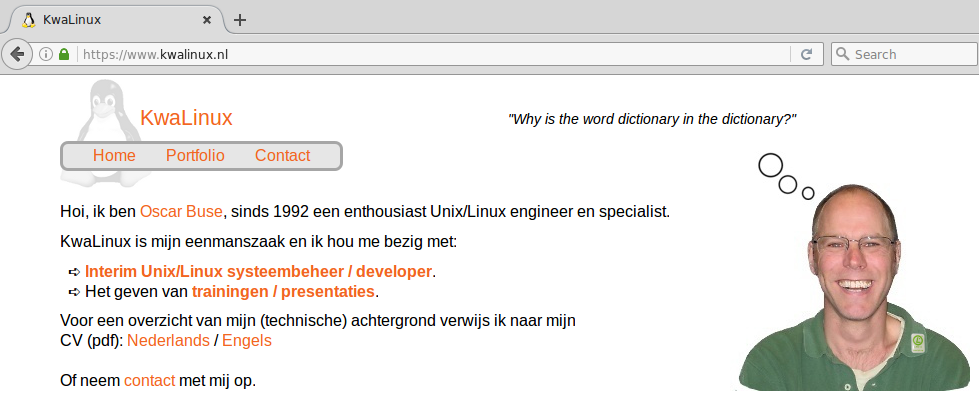
\includegraphics[width=10cm]{kwalinux.png}
\begin{itemize}
	\item Freelance Linux systeembeheer.
	\item Freelance Linux docent.
\end{itemize}
\end{styleframe}

\subsection{Over Meetup Linux Usergroup Nijmegen}
\begin{styleframe}
    \frametitle{Meetup Linux Usergroup Nijmegen}
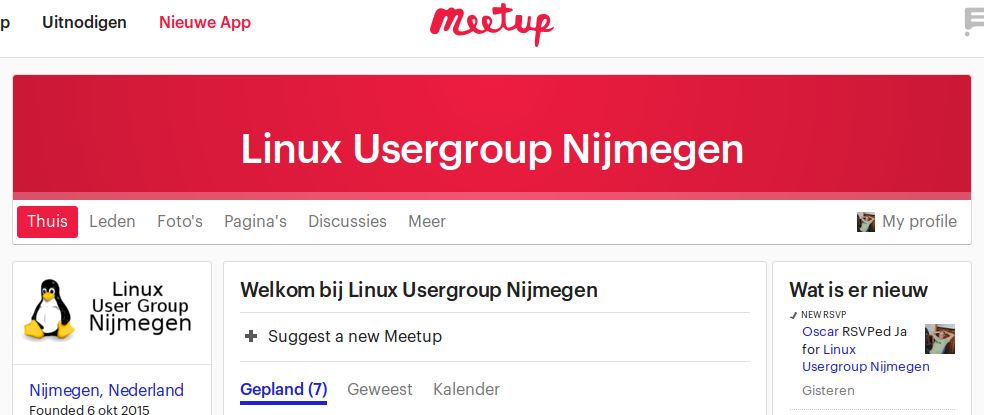
\includegraphics[width=10cm]{linuxnijmegen_meetup.png}
\begin{itemize}
	\item www.linuxnijmegen.nl (alle presentaties)
	\item Elke 2de dinsdag van de maand van 20:00 - 22:30. De klinker, van Broeckhuysenstraat 46, Nijmegen. 
\end{itemize}
\end{styleframe}

\subsection{Overzicht}
\begin{styleframe}
	\frametitle{Overzicht}
\begin{itemize}
	\item Inleiding en terminologie (SELinux modes, SELinux policy en SELinux access control)
	\item Lastig?
	\item Configuratie
	\item Werkwijze en 2 voorbeelden
	\item Concluderend
	\item Referenties
\end{itemize}
\end{styleframe}

\section{Inleiding en terminologie}
\subsection{Wat is SELinux?}
\begin{styleframe}
	\frametitle{Wat is SELinux?}
\begin{itemize}
	\pause
	\item project van de NSA en de SELinux community voor extra beveiliging bovenop het standaard Linux permissie systeem.
	\pause
	\item Mandators Access Control (MAC): het systeem bepaald de {\it policy}. Dit itt DAC (Discretionary Access Control: toegang gebasseerd op de {\it discretie} van de eigenaar).
	\pause
	\item Betere scheiding van rechten, betere bescherming tegen bv. fouten in software (privilege escalation).
	\pause
	\item SELinux data (de {\it security context}) is opgeslagen in de {\it extra attibutes} ruimte van de inode (sinds ext3, ook in xfs). Vaak zichtbaar met optie -Z bij bv. ls, id, ... Of -M bij ps.
	\pause
	\item {\it policies} bepalen wat is toegestaan (straks meer over policies).
\end{itemize}
\end{styleframe}

\subsection{SELinux modes}
\begin{styleframe}
    \frametitle{SELinux modes}
Er zijn drie modes (toestanden) waarin SELinux zich kan bevinden:
\begin{itemize}
	\pause
	\item enforcing (aan). Tegenwoordig default op in elk geval Fedora, CentOS en RedHat.
	\pause
	\item permissive (uit, wel logging)
	\pause
	\item disabled (uit)
\end{itemize}
Commandos / config:
\begin{itemize}
	\pause
	\item sestatus: toont huidige mode
	\pause
	\item setenforce: set mode (van/naar disabled: reboot)
	\pause
	\item file: /etc/sysconfig/selinux
\end{itemize}
\end{styleframe}

\subsection{SELinux {\bf algemene} policy}
\begin{styleframe}
	\frametitle{SELinux policy}
\pause
SELinux kent meerdere {\bf algemene} security policies, de bekendste:
\begin{itemize}
	\pause
 	\item targeted - all\'e\'en van toepassing op specifieke targets (daemons). Denk aan httpd, named, mysqld, dhcpd, nscd, ... \\
Users zijn niet beperkt ({\it unconfined}). \\
Dit is de default.
	\pause
	\item strict - Users ook aan policy onderhevig (confined). Is niet meer (sinds FC9) : opgenomen in de meer strict geworden targeted policy.
	\pause
	\item minimum - alleen SELinux voor specifiek aangegeven processen (om te experimenteren).
	\pause
	\item mls - zet Multi Level Security aan. Extra packages zijn nodig (o.a. selinux-policy-mls). Zet je niet ''zomaar'' aan.
\end{itemize}
\end{styleframe}

\subsection{SELinux access control}
\begin{styleframe}
    \frametitle{SELinux access control}
\pause
Als eerder vermeld: SELinux valt in de categorie MAC (itt DAC). Verder maakt SELinux in de {\bf targeted policy} standaard gebruik van:
\begin{itemize}
	\item Type Enforcement: security op basis van het type van ''subjects'' (processen), ''access'' (allow) en het type van ''objects'' (files, dirs, sockets, ...)".\\
Dit is de default in de SELinux targeted policy.
\end{itemize}
\pause
Andere typen access control die mogelijk zijn met SELinux maar niet standaard enabled (en geconfigureerd) zijn:
\begin{itemize}
	\item RBAC - Role based access control.
	\pause
	\item MCS/MLS - Multi Category (Sales, Tech, Staff) / Multi Level Security (Topsecret, Secret, Classified). Vooral MLS is meer voor militaire doeleinden en minder geschikt voor Linux servers..
\end{itemize}
%\pause
%Overige begrippen: \\
%{\tt \# ls -lZ f1
%-rw-r--r--. root root unconfined\_u:object\_r:admin\_home\_t:s0 f1
%\# id -Z
%unconfined\_u:unconfined\_r:unconfined\_t:s0-s0:c0.c1023}
%
%\begin{itemize}
%	\item users, roles, types (subjects (proces) types , object (file, dir, socket, ...) types), categorie\"en  en {\it levels}
%\end{itemize}
\end{styleframe}

\section{Lastig?}
\begin{styleframe}
    \frametitle{Lastig?}
\begin{itemize}
\pause
\item In theorie is SELinux best complex: er kan veel met SELinux (denk ook aan RBAC, MCS/MLS)
\pause
\item Valt mee in de praktijk:
	\begin{itemize}
	\pause
	\item All{\'e}{\'e}n {\it Type Enforcement} (TE), als onderdeel van MAC:
	''mag proces van type naam\_t iets (lezen, schrijven, executen, ...) met object van type naam\_t?'' \\
	%Uitzondering: unconfined types (unconfined\_t): SELinux is {\bf niet} van toepassing.
	\pause
    \item Default een {\it targeted} policy: all\'e\'en voor bepaalde daemons (httpd, dhcpd, ncsd, ...) geldt Type Enforcement.
	\pause
	\item Daemons komen standaard met gangbare default policy modules: zelf veelal geen policies te wijzigen/maken.
	\pause
	\item Users runnen standaard ''unconfined'' (SELinux niet van toepassing).
	\pause
	\item Voor het geval je wel zelf policies moet verzinnen zijn er veel hulpmiddelen (straks meer).
	\end{itemize}
\end{itemize}
\end{styleframe}

\begin{styleframe}
    \frametitle{in een plaatje}
 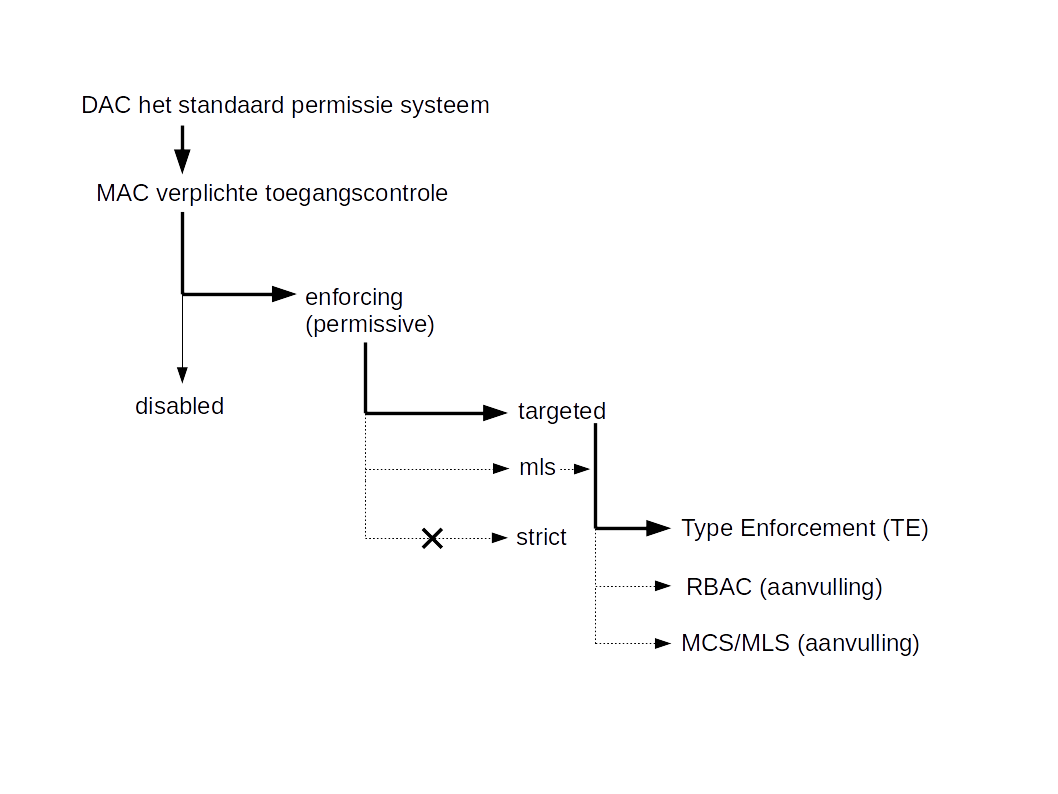
\includegraphics[width=300px]{samenvatting.png}
\end{styleframe}

\section{Configuratie}
\begin{styleframe}
    \frametitle{Configuratie}
\pause
\begin{itemize}
	\item /etc/sysconfig/selinux (mode, type algemene policy)
	\pause
	\item file labeling configuratie ({\it security contexts}): /etc/selinux/targeted/contexts/files/
	\pause
	\item pre-compiled policy modules voor veelvoorkomende toepassingen (\*.pp files): /etc/selinux/targeted/modules
Bv.: apache.pp, lvm.pp, ...
\end{itemize}
\end{styleframe}

\section{Praktisch}
\subsection{Werkwijze en tooling}
\begin{styleframe}
    \frametitle{Werkwijze en tooling}
\begin{itemize}
	\pause
	\item  Hoe weet je nu of een policy-rule bestaat voor bepaalde types?\\
	\pause
	{\scriptsize
	{\tt \# sesearch -Ad -s httpd\_t -t httpd\_sys\_content\_t -c file}}
	\pause
	\item Wat als je de policy wilt aanpassen of toevoegen? 
	\begin{itemize}
		\pause
		\item {\tt semodule\_unpackage}: maar niet de bedoeling dat je de default policies wijzigt...wordt ontmoedigd
		\pause
		\item {\tt booleans}: verander policy runtime (en ook permanent) met logische variabelen (on/off).
		\begin{itemize}
			\item getsebool -a : toont alle logische variabelen
			\item setsebool : set een logische variabele (-P : maak de setting permanent)
		\end{itemize}
		\pause
		\item {\tt semanage}: config policies zonder de default policy te wijzigen.
		\item Maak een module (pas op)
	\end{itemize}
\end{itemize}
\end{styleframe}

%\begin{styleframe}
%    \frametitle{Voorbeeld scenario: {\it confine} de user}
%Default zijn users (en dus user processen) niet beperkt ({\it confined}) door SELinux: \\
%{\tt ~$ id
%uid=1000(oscar) gid=1000(oscar) groups=1000(oscar) context=unconfined\_u:unconfined\_r:unconfined\_t:s0
%}
%
%Door de Linux-user aan een andere SELinux-user te koppelen wordt je nogal beperkt: \\
%{\tt # semanage login -m -s user\_u oscar}
%Of nog meer beperkt: \\
%{\tt # semanage login -m -s guest\_u oscar}
%\end{styleframe}

\subsection{Praktijkvoorbeeld 1}
\begin{styleframe}
    \frametitle{Voorbeeld scenario 1: een apart upload-dir}
Stel je hebt een boel ruimte gecre{\"e}erd onder {\tt /opt/upload/} waar de apache daemon mag schrijven: \\
~\\
\tiny
{\tt drwx------. apache apache unconfined\_u:object\_r:{\bf usr\_t}:s0 upload} \\
\pause
~\\
\small
Gebruik {\tt /var/log/audit/audit.log} om te kijken wat er mis gaat: \\
{\tt tail -f /var/log/audit/audit.log | grep denied} \\
{\bf Let op:} niet alles wordt standaard gelogt..! Zie waarde {\tt Dontaudit} met het commando {\tt seinfo}. \\
SELinux {\bf alles} laten loggen met: {\tt semodule -BD} \\
Wel weer terugzetten ({\tt semodule -B}) na troubleshooten. \\
\pause
~\\
De dir is van type {\bf usr\_t} maar voor apache moet deze van type {\bf httpd\_sys\_rw\_content\_t} zijn: \\
~\\
\tiny
{\tt semanage fcontext -m -t {\bf httpd\_sys\_rw\_content\_t} '/opt/upload(/.*)?'} \\
%\hspace{7pt} '/opt/upload(/.*)?'} \\
{\tt restorecon -Rv /opt/upload}
\end{styleframe}


\subsection{Praktijkvoorbeeld 2}
\begin{styleframe}
    \frametitle{Voorbeeld scenario 2: maak een module}
BackupPC is een handige grafische schil om rsync voor het maken van backups. \\
Er is geen standaard policy voor dus die moeten we zelf maken. \\
\pause
De stappen:
\footnotesize
\begin{itemize}
	\item definieer de type-labeling (file context):
	\footnotesize
	\begin{itemize}
		\footnotesize
		\item files onder /vol/grote\_patitie/BackupPC moeten benaderbaar zijn voor de webserver. Daartoe moeten ze van type
httpd\_sys\_content\_t zijn: \\
		\footnotesize
		{\tt \# semanage fcontext -a -t httpd\_sys\_content\_t  \\
		\hspace{7pt} '/vol/grote\_patitie/BackupPC(/.*)?' \\
		\# restorecon -Rv /vol/grote\_partitie/BackupPC} \\
		\footnotesize
		\pause
		\item onder /var/log/BackupPC moet de webserver kunnen loggen. Daartoe moeten de files van type httpd\_log\_t zijn: \\
		\footnotesize
	{\tt \# semanage fcontext -a -t httpd\_log\_t \\
	\hspace{7pt} '/var/log/BackupPC(/.*)?' \\
	\# restorecon -Rv /var/log/BackupPC/}
	\end{itemize}
\end{itemize}
\end{styleframe}

\begin{styleframe}
    \frametitle{Voorbeeld scenario 2: BackupPC}
Vaak nog niet genoeg..
\begin{itemize}
	\item Kijk naar denied regels in {\tt /var/log/audit/audit.log} en stop in file {\tt backuppc.txt}
	\pause
	\item Maak van opgespaarde denied regels policy rules (met audit2allow): \\
	\footnotesize
	{\tt cat backuppc.txt  | audit2allow -M backuppc} \\
	\pause
	Dit geeft:
	\begin{itemize}
		\item De Type Enforcement rules (ascii): {\tt backuppc.te}
		\pause
		\item Het binaire policy file met de type enforcement allow rules: {\tt backuppc.pp}
	\end{itemize}
	\pause
	\item De nieuwe policy rules installeren: {\tt \# semodule -i backuppc.pp}
\end{itemize}
\pause
{\bf Let wederom op:} niet alles wordt standaard gelogt..! Zie waarde {\tt Dontaudit} met het commando {\tt seinfo} en run evt. {\tt semodule -BD}. \\
{\bf Pas voor introduceren ruime of anderszins ongebruikelijke policies..}
\end{styleframe}

\begin{styleframe}
    \frametitle{Voorbeeld scenario 2 - extra}
Het .te file is ook te gebruiken om een policy handmatig te maken/onderhouden. Bv. als je later toch nog een
''denied'' regel in de audit.log tegenkomt. De stappen:
\pause
\begin{itemize} 
	\item voeg bv. een extra allow regel toe (lastig! {\tt audit2allow} is er niet voor niets..)
	\pause
	\item denk ook aan de ''required'' items en verhoog het versie nummer van je module
	\pause
	\item Genereer een binary module: \\ 
	{\scriptsize {\tt \# checkmodule -o backuppc.mod backuppc.te -m}} \\
	\pause
	\item Genereer een module package: \\
	{\scriptsize {\tt \# semodule\_package -o backuppc.pp -m backuppc.mod}}
	\pause
	\item {\tt \# semodule -i backuppc.pp}
\end{itemize}
\end{styleframe}

\section{Concluderend}
\begin{styleframe}
    \frametitle{Concluderend}
\begin{itemize}
	\item SELinux geeft meer fijnmazige controle.
	\pause
	\item Introduceert complexiteit. In veel (standaard) gevallen opgevangen door klant-en-klare policies en all\'e\'en Type Enforcement.
	\pause
	\item Minder kans op {\it privilege escalation}.
	\pause
	\item Door systeem geforceerd (niet gebasseerd op de {\it discretie} van de eigenaar zoals bij het normale Linux permissiesysteem).
	\pause
	\item Kan nog veel meer mee (RBAC, MCS/MLS (wordt dan al snel complexer)).
	\pause
	\item Geen vervanging van andere security maatregelen, alleen iets extra's
	\pause
	\item Bij ondeskundig gebruik (makkelijk met audit2allow!) kans op afzwakken security model (er is natuurlijk nog wel altijd nog het normale permissiesysteem).
\end{itemize}
\end{styleframe}

\section{Referenties}
\begin{styleframe}
    \frametitle{Referenties}
Enkele url's met informatie: \\
~\\
\footnotesize
\url{http://docs.fedoraproject.org/en-US/Fedora/25/html/SELinux\_Users\_and\_Administrators\_Guide/}
~\\
~\\
\url{http://wiki.centos.org/HowTos/SELinux}
~\\
~\\
\url{https://debian-handbook.info/browse/stable/sect.selinux.html}
~\\
~\\
\url{http://stopdisablingselinux.com/}
\end{styleframe}
